\documentclass[a4paper]{article}

\usepackage[utf8]{inputenc}
\PassOptionsToPackage{hyphens}{url} % zodat url's ook afgekapt worden
\usepackage{hyperref}
\usepackage[dutch]{babel}
\usepackage{graphicx}
\graphicspath{{img/}}
\usepackage{algorithm}
\usepackage{algorithmic}
\usepackage[toc,page]{appendix}
\usepackage{mathtools}
\usepackage{tocbibind}
\usepackage{float}
\usepackage{framed}
\usepackage{parskip}
\usepackage{listings}
\usepackage{color}
\usepackage{pdfpages}
\usepackage{pdflscape}
\usepackage{todonotes}
\usepackage{tabularx}
\usepackage{usecases}
\usepackage{enumitem}


\begin{document}
%%%%%%%%%%%%%%%%%%%%%%%%%%%%%%%%%%%%%%%%%
% University Assignment Title Page 
% LaTeX Template
% Version 1.0 (27/12/12)
%
% This template has been downloaded from:
% http://www.LaTeXTemplates.com
%
% Original author:
% WikiBooks (http://en.wikibooks.org/wiki/LaTeX/Title_Creation)
%
% License:
% CC BY-NC-SA 3.0 (http://creativecommons.org/licenses/by-nc-sa/3.0/)
% 
% Instructions for using this template:
% This title page is capable of being compiled as is. This is not useful for 
% including it in another document. To do this, you have two options: 
%
% 1) Copy/paste everything between \begin{document} and \end{document} 
% starting at \begin{titlepage} and paste this into another LaTeX file where you 
% want your title page.
% OR
% 2) Remove everything outside the \begin{titlepage} and \end{titlepage} and 
% move this file to the same directory as the LaTeX file you wish to add it to. 
% Then add \input{./title_page_1.tex} to your LaTeX file where you want your
% title page.
%
%%%%%%%%%%%%%%%%%%%%%%%%%%%%%%%%%%%%%%%%%

%----------------------------------------------------------------------------------------
%	PACKAGES AND OTHER DOCUMENT CONFIGURATIONS
%----------------------------------------------------------------------------------------
\begin{titlepage}
\pagestyle{empty}
\newcommand{\HRule}{\rule{\linewidth}{0.5mm}} % Defines a new command for the horizontal lines, change thickness here

\center % Center everything on the page
 
%----------------------------------------------------------------------------------------
%	HEADING SECTIONS
%----------------------------------------------------------------------------------------

\textsc{\LARGE Universiteit Hasselt}\\[1.5cm] % Name of your university/college
\textsc{\Large Software Engineering}\\[0.5cm] % Major heading such as course name
\textsc{\large Requirements analyse }\\[0.5cm] % Minor heading such as course title
% \textsc{\LARGE Modulo}\\[0.5cm] % Minor heading such as course title

%----------------------------------------------------------------------------------------
%	TITLE SECTION
%----------------------------------------------------------------------------------------

\HRule \\[0.4cm]
%{ \huge \bfseries Managementsysteem \\ Deeltijds Onderwijs }\\[0.2cm] % Title of your document
{ \huge \bfseries Modulo \\ \vspace{-0.4em} ----- \vspace{-0.4em}\\ Managementsysteem \\ Deeltijds Onderwijs }\\[0.2cm] % Title of your document
\HRule \\[1.5cm]
 
%----------------------------------------------------------------------------------------
%	AUTHOR SECTION
%----------------------------------------------------------------------------------------

\begin{minipage}{0.4\textwidth}
\begin{flushleft} \large
\emph{Auteurs:}\\
Vincent \textsc{Drozdzyniak} % Your name
Hendrik \textsc{Lievens} \\ 
Martijn \textsc{Maes} \\
Reinaert \textsc{Van de Cruys} \\
Michiel \textsc{Vanmunster} \\
Jens \textsc{Vannitsen}
\end{flushleft}
\end{minipage}
~
\begin{minipage}{0.4\textwidth}
\begin{flushright} \large
% \emph{Promotor:} \\
% Prof. dr. Frank \textsc{Neven}\\ % Supervisor's Name
% \vspace{4mm}
\emph{Begeleider:} \\
Robin \textsc{Marx}
\end{flushright}
\end{minipage}\\[2.5cm]

% If you don't want a supervisor, uncomment the two lines below and remove the section above
%\Large \emph{Author:}\\
%John \textsc{Smith}\\[3cm] % Your name


%----------------------------------------------------------------------------------------
%	DATE SECTION
%----------------------------------------------------------------------------------------

{\large 17 maart 2016}\\[2cm] % Date, change the \today to a set date if you want to be precise

%----------------------------------------------------------------------------------------
%	LOGO SECTION
%----------------------------------------------------------------------------------------


\includegraphics[width=0.4\textwidth]{UH_logo}\\[2cm] % Include a department/university logo - this will require the graphicx package
 
%----------------------------------------------------------------------------------------

\vfill % Fill the rest of the page with whitespace

\end{titlepage}

\tableofcontents
\newpage

\section{Preface}
Dit document is bedoeld voor het personeel van het Technisch Instituut Heilig Hart te Hasselt \cite{TIHH} zijnde de opdrachtgevers, het onderwijsteam en het ontwikkelingsteam van Modulo. In dit document worden alle vereisten van het softwarepakket geanalyseerd.


\section{Inleiding}
Modulo is een Managementsysteem voor het Deeltijds Onderwijs (MDO) dat gebruikt kan worden in alle onderwijsinstellingen waar het Deeltijds Beroepssecundair Onderwijs (DBSO) \cite{DBSO} als onderwijsvorm wordt gehanteerd. Dit omvat alle Centra voor Deeltijds Onderwijs (CDO) \cite{CDO} alsook het Syntra-netwerk \cite{Syntra}.

Is een onderwijsvorm waarin leerlingen leren op school combineren met leren op werkplekken.  Een lesweek bestaat uit 8 uur BGV en 7 uur PAV, de rest van de tijd brengen de leerlingen doorop de werkvloer. Een opleiding duurt drie jaar. Tijdens het vak PAV moeten de leerlingen voor iedere graad doelstellingen verwerven die voorgelegd zijn door de overheid (leerplan). Wanneer men voor alle graden, alle doelstelling verworven heeft krijgt de leerling het diploma secundair onderwijs. Tijdens de BGV vakken leert men een beroep aan. Om een beroep uit te kunnen oefenen heb je het certificaat nodig van dat beroep. Dit certificaat kan je verkrijgen tijdens de BGV lessen. Iedere certificaat is opgedeeld in deelcertificaten en ieder van deze deelcertificaten bestaat uit competenties. Je verkrijgt een certificaat wanneer je alle deelcertificaten verworven hebt. Een deelcertificaat verkrijg je als je alle competenties van dit certificaat verworven hebt. Met de invoering van het duaal leren \cite{Duaal_leren} zal Modulo ook in alle beroeps- en technische richtingen gebruikt kunnen worden. \todo{ NIEUW jens: eens nalezen aub}

In sectie \ref{sec:general_descr} wordt allereerst een algemeen beeld gegeven van de werking en het precieze doel van Modulo. Vervolgens worden in sectie \ref{sec:user_req} alle vereisten van het softwarepakket tegenover de gebruiker besproken. Er wordt een uitgebreide lijst van vereiste functionaliteiten gegeven, alsook een analyse van het gebruik, de mogelijkheden voor ondersteuning en de juridische aspecten. Sectie \ref{sec:systeemarchitectuur} biedt een uiteenzetting van de gekozen technologieën om het softwarepakket te implementeren en in sectie \ref{sec:use_cases} wordt dieper ingegaan op de concrete stappen die verschillende types gebruikers moeten doorlopen om bepaalde acties te ondernemen. In de appendices tenslotte kunnen mockups gevonden worden die tonen hoe Modulo er voor de gebruiker uitziet.



\section{Woordenlijst} % voor de klant
\def\arraystretch{1.8}
\begin{tabularx}{\textwidth}{l | X}
    Term & Definitie \\
    \hline \hline
    MDO &`Managementsysteem voor het Deeltijds Onderwijs' is het antwoord op de vraag ``Wat is Modulo?''. Het is een softwarepakket voor het beheren van de gegevens van leerlingen binnen het DBSO. \\
    \hline
    DBSO & `Deeltijds Beroepssecundair Onderwijs', of kortweg `deeltijds onderwijs', is een onderwijsvorm waarin leerlingen leren op school combineren met leren op werkplekken. Een lesweek bestaat uit 8 uur BGV en 7 uur PAV, de rest van de tijd brengen de leerlingen door op de werkvloer. \cite{DBSO} \\
    \hline
    CDO & `Centra voor Deeltijds Onderwijs' zijn scholen die DBSO als onderwijsvorm hanteren. De opdrachtgever voor Modulo, het Technisch Instituut Heilig Hart te Hasselt \cite{TIHH}, is hier een voorbeeld van. \cite{CDO} \\
\end{tabularx}

\newpage
\begin{tabularx}{\textwidth}{l | X}
    Term & Definitie \\
    \hline \hline
    BGV & `Beroepsgerichte Vorming' is het vak binnen het DBSO dat alle beroepsspecifieke competenties voor een opleiding omvat en zo de leerlingen alle kennis en vaardigheden bijbrengt die ze op de werkvloer nodig hebben. \\
    \hline
    PAV & `Project Algemene Vorming' of `Project Algemene Vakken' is het vak binnen het DBSO dat in alle doelstellingen van de 2de en 3de graad omvat, zodat de leerlingen hun diploma secundair onderwijs kunnen behalen. \\
    \hline
    Competentie & Het certificaat dat door middel van BGV verkregen kan worden, bestaat uit een verzameling deelcertificaten. Ieder deelcertificaat bestaat uit een lijst van competenties, vastgelegd door de Vlaamse overheid, die de leerlingen allemaal moeten halen om het deelcertificaat te verkrijgen. Een deelcertificaat kan op andere deelcertificaten voortbouwen, die dan ook in volgorde behaald moeten worden. \cite{Competenties} \\
    \hline
    Doelstelling & Een doelstelling is een module binnen PAV die bepaald wordt door de eindtermen voor het secundair onderwijs van de Vlaamse overheid. leerlingen moeten alle doelstellingen halen alvorens ze het diploma secundair onderwijs kunnen ontvangen. Een doelstelling kan bestaan uit andere doelstellingen, die dan opnieuw allemaal behaald moeten worden. \cite{Doelstellingen} \\
    \hline
    A,I,V & A (aangeboden), I (ingeoefend) en V (verworven) zijn de drie mogelijke toestanden die een aangeboden competentie of doelstelling op een bepaalde dag toegewezen kan krijgen. Indien de leerkracht `verworven' invult, betekent dit dat de leerling heeft aangetoond de competentie of doelstelling te beheersen, `ingeoefend' betekent dat de leerling inzet heeft getoond om de competentie of doelstelling te behalen, en `aangeboden' betekent dat de leerling zich niet heeft ingezet of afwezig was. Binnen het TIHH, de opdrachtgever van dit softwarepakket, wordt een competentie of doelstelling pas als behaald beschouwd wanneer de leerling er drie keer een V (verworven) voor heeft gescoord, op verschillende dagen. Daarna wordt de leerling niet meer op de betreffende competentie of doelstelling beoordeeld.
\end{tabularx}


\newpage
\section{Algemene beschrijving}  \label{sec:general_descr}% voor de klant
Modulo is een softwarepakket voor het beheren van de gegevens van leerlingen binnen scholen die het DBSO als onderwijsvorm toepassen. Er kan onder meer een klassenbestand worden bijgehouden, leerlingen kunnen worden geëvalueerd en overzichtelijke rapporten kunnen worden uitgeprint. Modulo is echter geen algemeen beheersysteem; het bevat bijvoorbeeld geen functionaliteit om financiën te beheren, of om beschikbaar en aan te kopen lesmateriaal bij te houden.

Modulo onderscheidt vier types gebruikers: beheerders, leerkrachten, leerlingen en ouders. Alle gebruikers hebben een webapplicatie ter beschikking waarin de volledige functionaliteit van het softwarepakket voor dat type gebruiker vertegenwoordigd is. Leerlingen en ouders hebben aanvullend toegang tot een Android applicatie, beschikbaar vanaf de Google Play Store.

Het softwarepakket bestaat uit acht modules:

\begin{enumerate}
    \item Gebruikersbeheer
    \item Beheer van graden en opleidingen
    \item Klassenbeheer
    \item Puntenbeheer
    \item Weergeven van voortgang van leerlingen
    \item Genereren van rapporten
    \item Werkgeversbeheer
    \item Genereren van werkgeverscontracten
\end{enumerate}
Modules 1 en 2 zijn enkel beschikbaar voor beheerders. Modules 3-8 zijn beschikbaar voor leerkrachten. Leerlingen en ouders beschikken enkel over module 5. Modulo is dus veruit het meest uitgebreid voor leerkrachten. De volgende paragrafen geven een algemeen beeld van de functionaliteiten van de verschillende modules. Voor een gedetailleerde stap-voor-stap beschrijving van de acties die gebruikers moeten nemen om bepaalde taken uit te voeren, kan sectie \ref{sec:use_cases} geraadpleegd worden.

De taak van beheerders is, in één woord, `systeembeheer'. Via de module `Gebruikersbeheer' kunnen zij gebruikers toevoegen, verwijderen, bewerken en op inactief zetten, en via de module `Beheer van graden en opleidingen' kunnen zij de eindtermen van de twee vakken binnen het DBSO, BGV en PAV, aanpassen. Beheerders kunnen ook opleidingen binnen BGV op inactief zetten, wanneer deze niet op de school worden aangeboden.

Leerkrachten kunnen allereerst klassen samenstellen, binnen BGV of PAV, waaraan zij les geven (module 3). Vervolgens kunnen zij binnen deze klassen per lesdag punten (A,I,V) aan leerlingen toekennen, met toevoeging van commentaar (module 4). Deze punten kunnen zij later ook opvragen in een scherm dat zowel algemene als gedetailleerde voortgang toont (module 5). Dit scherm kan ook worden omgezet in de vorm van een rapport en worden afgedrukt (module 6). Daarnaast kunnen leerkrachten de werkgeversdatabank, een lijst van alle werkgevers waar leerlingen hun praktijkdagen kunnen bij doorbrengen, bewerken, en kunnen ze leerlingen aan werkgevers koppelen (module 7). Tenslotte kunnen ze ook contracten tussen leerlingen en werkgevers genereren, op basis van sjablonen, en deze afdrukken om te laten ondertekenen (module 8).

Leerlingen en ouders kunnen enkel respectievelijk hun eigen voortgang of die van hun kinderen kunnen bekijken (module 5). Indien ouders meerdere kinderen op de school hebben, kunnen zij kiezen uit een lijst van kinderen om de voortgang van te bekijken. De voortgang kan bekeken worden zowel via de web- als via de mobiele applicatie. Het idee van de mobiele applicatie is om het laagdrempeliger te maken voor ouders en leerlingen om regelmatig de voortgang te bekijken.



\newpage
\section{User requirements}  \label{sec:user_req}% voor de klant

\todo{Michiel: opsplitsen in logische gehelen}

\subsection{Functionele requirements}
\begin{enumerate}[label=F\arabic*]
% algemeen
\item Het systeem moet toelaten om gebruikers toe te voegen en te verwijderen. Hierbij wordt een account voor de gebruiker aangemaakt (of verwijderd).
\item Het systeem moet toelaten om aan een gebruiker een rol (leerkracht, leerling, beheerder, ouder) toe te kennen.
\item Het systeem moet toelaten om in te stellen of een gebruiker al dan niet actief is. Dit houdt in dat de gebruiker niet meer in het systeem voorkomt, maar alle persoonlijke info opgeslagen blijft in het systeem, voor het geval deze terug actief zou worden \footnote{Ter motivatie hiervan vermelden we dat het in het deeltijds onderwijs voorvalt dat leerlingen zich gedurende hun opleiding uitschrijven. Maar dan later, wanneer bv. blijkt dat ze geen werk vinden, ze alsnog hun opleiding willen verder zetten.}.
\item \label{itm:pers_info} Het systeem moet toelaten om de persoonlijke informatie van een leerling \footnote{Deze info bestaat uit: naam, voornaam, geboortedatum, geboorteplaats, nationaliteit, rijksregisternummer, straat, nummer, bus, postcode, gemeente, gsm, telefoon ouders, rekeningnummer. We houden deze info alleen bij voor leerlingen omdat de school apart de gegevens van het personeel bijhoudt en we het telefoonnummer van de ouders bij de leerling bijhouden.} aan te passen. 
\item \label{itm:inschr_info} Het systeem moet toelaten om inschrijvingsgerelateerde informatie \footnote{Dit houdt in: graad met PAV-klas, opleiding met BGV-klas, en datum van inschrijving.} van een leerling aan te passen.
\item \label{itm:account_info} Het systeem moet de beheerder toelaten om accountgerelateerde informatie \footnote{Dit zijn gebruikersnaam, wachtwoord en e-mailadres.} van een gebruiker aan te passen.
\item Het systeem moet toelaten om kinderen te koppelen aan ouders.
\item Het systeem moet toelaten om PAV- en BGV-klassen toe te voegen, te verwijderen en te bewerken.  
% PAV
\item Het systeem moet de PAV-doelstellingen per graad, opgelegd door de overheid, voorzien. De doelstellingen in deze lijst kunnen bewerkt en verwijderd worden door de beheerder, en er kunnen manueel extra doelstellingen worden toegevoegd. \footnote{De motivatie achter het manueel aanpassen van doelstellingen is dat deze doelstellingen door de overheid vaak moeilijk of onduidelijk verwoord zijn.}
\item Het systeem moet de BGV-competenties per deelcertificaat per opleiding, opgelegd door de overheid, voorzien. De competenties in deze lijst kunnen bewerkt en verwijderd worden door de beheerder, en er kunnen manueel extra competenties worden toegevoegd.
\item Het systeem moet toelaten om van een opleiding in te stellen of deze al dan niet door de school wordt aangeboden \footnote{De overheid lijst zo'n 150 opleidingen op, maar een school zal er typisch slechts zo'n 20 aanbieden}.
\item Het systeem moet toelaten om een vakthema of remediëringstaak aan een aantal leerlingen van een klas toe te kennen. Deze worden opgebouwd uit doelstellingen. Indien alle leerlingen gekozen worden spreekt men van een vakthema, anders van een remediëringstaak.
% BGV
\item Het systeem moet toelaten om een beheerder BGV klassen aan te laten maken, deze klassen stellen de verschillende opleidingen voor (bv. Mestselaar bestaat uit 2klassen: Metselaar1 en Metselaar2).
\todo{Nieuw Martijn: beheerder maakt BGV klassen aan}
\item Het systeem moet toelaten om een score (A,I,V) (zie woordenlijst) toe te kennen aan een doelstelling binnen een vakthema, voor een leerling.  % PAV
\item Het systeem moet toelaten om een score (A,I,V) toe te kennen aan een competentie binnen een deelcertificaat, voor een leerling.  % BGV
\item Het systeem moet automatisch het behalen van een competentie blokkeren voor een leerling, indien deze reeds drie maal verworven (score V) werd.  % 3x verwerven == behaald
\item Het systeem moet het verloop van het jaar kunnen weergeven. Dit overzicht toont voor één leerling de behaalde scores (A, I, V) per competentie per week.
\item Het systeem moet toelaten om een beschrijving te geven bij het verwerven van een competentie of doelstelling, en de datum waarop deze verworven werd in te stellen.
\item Het systeem moet toelaten om een ingevuld rapport te genereren, voor een leerling.
\item Het systeem moet toelaten om de houdingen/attitudes van de leerlingen in te vullen. Op het einde van een les, bijvoorbeeld, kan de leerkracht een punt (slecht, matig, goed) toekennen aan iedere leerling van de klas.
% algemeen
\item Het systeem moet toelaten om informatie over de school \footnote{Deze info bestaat uit: naam van de school, naam van de directeur, logo, straat, nummer, postcode, gemeente, telefoonnummer, email, website.} aan te passen.
\item \label{itm:werkgever_info} Het systeem moet leerkrachten toelaten om werkgevers waar de school mee samenwerkt\footnote{In het deeltijds onderwijs werkt een school vaak samen met bedrijven. Info over deze bedrijven wordt gebruikt in item \ref{itm:werkgever1} en \ref{itm:werkgever2}. Een werkgever heeft geen account binnen Modulo.} toe te voegen en te verwijderen, en informatie over een werkgever\footnote{Dit zijn: bedrijfsnaam, juridische vorm, BTW nummer, RSZ nummer, IPK nummer, PC nummer, erkenning PC, adres, telefoon, fax, email, rekeningnummer, verantwoordelijke (persoon die de student in dienst neemt: naam, adres, telefoon, email).} aan te passen.
\item Het systeem moet toelaten om voor een werkgever in te stellen of er momenteel al dan niet een actieve samenwerking is. Dit houdt in dat de werkgever al dan niet kan toegewezen worden aan een leerling (zie \ref{itm:werkgever1}). \footnote{De werkgever zal niet op ieder moment studenten kunnen te werk stellen.}
% werkgevers zijn geen gebruikers
\item \label{itm:werkgever1} Het systeem moet toelaten aan een leerkracht om een werkgever (waar de school mee samenwerkt) aan een leerling toe te wijzen.
\item \label{itm:werkgever2} Het systeem moet toelaten om een contract te genereren voor de samenwerking tussen leerling en werkgever. In het gegenereerde contract moet alle info over de leerling en de werkgever automatisch worden ingevuld.
\item Het systeem moet bijhouden (loggen) wanneer een ouder of leerling de voortgang bekijkt.
\end{enumerate}

% extra's worden in 'systeemevolutie' besproken


\subsection{Usability}
De gebruikersinterface is een uitgesproken belangrijk onderdeel van Modulo, want aangezien het om een managementsysteem gaat, staat of valt de bruikbaarheid van het softwarepakket met diens overzichtelijkheid. Voor alle types gebruikers zijn duidelijkheid en een vlotte werking essentieel, omdat ze vaak met lange lijsten van complexe gegevens werken, zoals de lijst van scores die een leerling behaald heeft, of de lijst van leerlingen in een klas. Ook consistentie is van belang, in het bijzonder omdat er zowel een web- als een mobiele applicatie beschikbaar is. Deze zijn eenvoudiger afwisselend te gebruiken indien hun design en werking vergelijkbaar zijn.

Om een vlotte werking te bevorderen, kunnen meerdere items tegelijk uit lijsten geselecteerd worden, waarna acties op alle geselecteerde items tegelijk kunnen worden uitgevoerd (bv. een score voor een bepaalde doelstelling of competentie kan aan meerdere leerlingen, of zelfs een hele klas, tegelijk worden toegekend). Ook biedt een zoekfunctie de mogelijkheid om snel specifieke items in een lijst terug te vinden.

Consistentie wordt bereikt door middel van eenzelfde design (kleurenschema, fonts en ontwerp van elementen) over de gehele web- en mobiele applicatie heen. Ook een consistente woordkeuze (bv. voortgang van leerlingen wordt steeds `voortgang' genoemd en niet soms `punten' of `resultaten') en een consistente layout (bv. knoppen om items in een lijst te bewerken, toe te voegen of te verwijderen kunnen steeds in dezelfde plaats op het scherm gevonden worden, of het nu om punten voor een vak of leerlingen in een klas gaat) dragen hiertoe bij.


\subsection{Reliability}
Zowel de web- als de mobiele applicatie zijn slechts interfaces naar de back-end. Bijgevolg is uptime van de back-end servers essentieel voor de reliability van het softwarepakket. Om die reden wordt hosting van deze servers uitbesteed aan een gespecialiseerd bedrijf met een hoge uptime garantie, dat deze taak vermoedelijk goedkoper en betrouwbaarder kan uitvoeren dan het ontwikkelingsteam zelf.


\subsection{Performance}
\todo{RAIL model toegevoegd}
Op het vlak van performantie zijn er geen specifieke vereisten, maar een vlotte werking van het softwarepakket is uiteraard belangrijk. Daarom moeten lange responstijden en merkbare laadtijden tot een minimum beperkt worden. Het ontwikkelingsteam profileert de performantie en voert optimalisaties door waar nodig en mogelijk. Volgens het RAIL performantie model \cite{RAIL}, moeten performantievertragingen beperkt worden tot 300ms - 1000ms. De gebruiker ervaart dan natuurlijke en progressieve voortgang van taken.


\subsection{Supportability}
Het softwarepakket moet makkelijk uitbreidbaar en eenvoudig te onderhouden zijn. In het geval van een onderwijshervorming moeten bijvoorbeeld met weinig moeite nieuwe opleidingen, doelstellingen en competenties kunnen worden toegevoegd (of verwijderd). De back-end van het softwarepakket draait op servers van een gespecialiseerd hosting bedrijf en blijft zo eenvoudig toegankelijk voor het ontwikkelingsteam, en de mobiele applicatie wordt geïnstalleerd vanaf de Google Play Store, waardoor ook daar eenvoudig updates doorgevoerd kunnen worden.


\subsection{Legal}
Het softwarepakket moet voldoen aan de privacy wetgeving, in het bijzonder betreffende de resultaten en persoonlijke informatie van de leerlingen. Ouders mogen enkel de gegevens van hun eigen kinderen kunnen bekijken en enkel aangemelde personeelsleden mogen gevoelige informatie, waaronder ook de rekeningnummers van leerlingen en werkgevers, kunnen opvragen.

De back-end van het softwarepakket draait op servers van een gespecialiseerd hosting bedrijf dat volledige privacy en een goede beveiliging garandeert, zowel fysiek als virtueel. Verbindingen tussen de back-end server en de web- of mobiele applicatie gebeuren steeds over HTTPS en bevatten steeds een ID om de identiteit van de gebruiker kenbaar te maken.

Het softwarepakket hoeft geen rekening te houden met de wetgeving rond contracten. Deze kunnen enkel gegenereerd worden vanaf sjablonen en vervolgens afgeprint, maar worden niet digitaal ondertekend noch opgeslagen.


\subsection{Operations}
Na de ingebruikname van Modulo worden de doelstellingen en competenties up-to-date gehouden. Concreet betekent dit het volgende: de overheid zou competenties van een opleiding of doelstellingen van een graad kunnen aanpassen, verwijderen of er toevoegen. Ook zou de overheid een nieuwe opleiding kunnen opstellen (met bijhorende competenties). Modulo zal zulke wijzigingen op maandelijks basis voor de klant updaten.




\newpage
\section{Systeemarchitectuur}  \label{sec:systeemarchitectuur} % NIET voor de klant
\todo{Motivatie aangepast bij Java en Angular}
Het softwarepakket bestaat uit 3 deelsystemen:

\begin{enumerate}
    \item Een centrale back-end, onzichtbaar voor de gebruiker.
    \item Een front-end als webapplicatie.
    \item Een front-end als mobiele applicatie.
\end{enumerate}

\begin{figure}[H]
  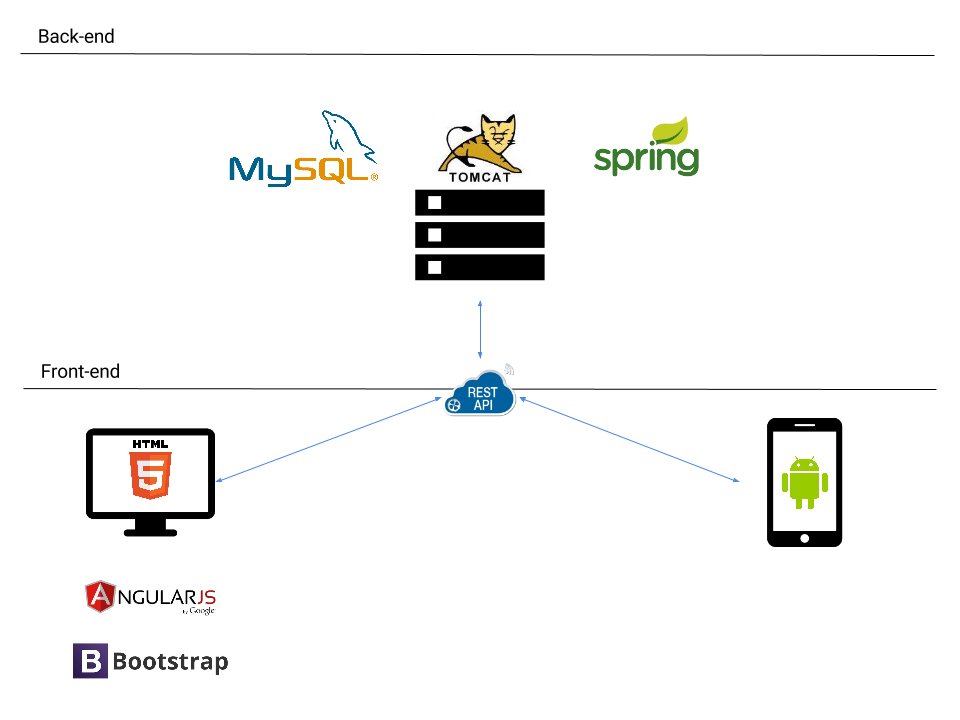
\includegraphics[width=\textwidth]{technologie_stack}
  \caption{Systeemarchitectuur}
  \label{fig:Systeemarchitectuur}
\end{figure}

De back-end wordt geïmplementeerd in Java, met behulp van het \textit{Spring Framework} \cite{Spring}. Voor de webapplicatie worden het \textit{AngularJS Framework} \cite{AngularJS} en het \textit{Bootstrap Framework} \cite{Bootstrap} gebruikt. De mobiele applicatie is beschikbaar voor het Android platform en wordt opnieuw in Java geïmplementeerd. De interactie tussen de front-end en back-end gebeurt door middel van zogenoemde \textit{RESTful} communicatie \cite{REST}. MySQL \cite{MySQL} dient als databasemanagementsysteem en wordt samen met de back-end gehost op een \textit{Tomcat} \cite{Tomcat} server.

\newpage
\subsection{Motivatie}
\begin{description}
    \item[Java] is een volwaardige objectgeoriënteerde programmeertaal. Het is een strongly typed programmeertaal die zich uitstekend leent voor business logic. Java beschikt over een groot aantal uitgebreide frameworks voor quasi alle denkbare toepassingen. We kiezen niet voor PHP, omdat deze taal niet voldoende object-georiënteerd is en weakly typed is. Java lijkt ook een betere keuze dan C\# wegens het cross-platform karakter van de taal.
    \item[MySQL] is een vrij te gebruiken relationeel databasemanagementsysteem. Dit is ook het databasesysteem waarmee we het ontwikkelingsteam het best bekend is.
    \item[Spring Framework] is  een antwoord op de kritiek die gericht is aan de werking van het klassieke Java EE. Een van de grote sterktes is de uitgebreide documentatie. Met behulp van Spring is men in staat om snel een API te ontwikkelen. Ook hebben we het Jersey Framework overwogen, maar kozen we toch voor Spring wegens alle andere extra componenten die het framework te bieden heeft (o.a. Spring Web, Spring Security en Spring Data).
    \item[Angular JS Framework] is een framework gebaseerd op JavaScript en dient als communicatiemiddel tussen back-end en front-end. Het is eenvoudig en handig voor snelle ontwikkeling van web pagina's. Ook is het makkelijk te combineren met HTML en CSS en is het compatibel met andere frameworks of libraries (bv. Bootstrap). We verkiezen AngularJS boven custom javascript om ons platform modulair, consistent en uitbreidbaar te houden.
    \item[Bootstrap Framework] is een van de meest populaire HTML, CSS en JavaScript frameworks gebruikt voor de ontwikkeling van responsieve webapplicaties. Bootstrap maakt front-end web ontwikkeling sneller en makkelijker, het is flexibel en het levert zowel op desktop- als op mobiele platformen mooie resultaten op. Omdat Bootstrap gebruik maakt van JQuery functionaliteit en JQuery niet optimaal samenwerkt met AngularJS, wordt er gebruik gemaakt van de eenvoudige Angular-UI \cite{AngularUI} Bootstrap bibliotheek. 
\end{description}

\clearpage


\todo{Iedereen: Belangrijkste use cases fully dressed}
\section{Use cases} \label{sec:use_cases}

%%%%%%%%%%%%%%%%%%%%%%%%%%%%%%%%%%%%%%%%%%%%%%%%%%%%%%%%%%%%%%%%%%%%%%%%%%%%%
%BEHEERDER
%%%%%%%%%%%%%%%%%%%%%%%%%%%%%%%%%%%%%%%%%%%%%%%%%%%%%%%%%%%%%%%%%%%%%%%%%%%%%

\subsection{Beheerder}


%Gebruikers toevoegen
\begin{usecase}
    \addtitle{Use Case 1}{Gebruiker toevoegen} 
    \additemizedfield{Primaire actor}{
    	\item Beheerder
    } 
    \additemizedfield{Stakeholders en interests}{ 
        \item Beheerder: Andere mensen toegang geven tot het systeem.
        \item Leerling: De leerling krijgt toegang tot het systeem.
        \item Leerkracht: De leerkracht krijgt toegang tot het systeem.
        \item Ouder: De ouder krijgt toegang tot het systeem.
    }
    \addfield{Preconditie}{
        De beheerder moet aangemeld zijn. De opleidingen en klassen moeten bestaan.
    }
    \addfield{Postconditie}{
        De gegevens over de gebruiker worden correct opgeslagen.
    }
    \addscenario{Hoofdscenario}{
        \item Beheerder kiest ``Gebruikersbeheer''.
        \item Het systeem geeft een lijst weer van alle gebruikers.
        \item Beheerder kiest ``Gebruiker toevoegen''.
        \item Systeem toont een dropdown waarmee de gebruikersrol dient ingesteld te worden.
        \item Beheerder kiest ``leerling'' als gebruikersrol.
        \item Systeem toont een leeg formulier waarin alle informatie over de leerling moet worden ingevuld. Dit zijn de persoonlijke, accountgerelateerde en inschrijvingsgerelateerde informatie (zie \ref{itm:pers_info}, \ref{itm:account_info} en \ref{itm:inschr_info}).
        \item Beheerder vult alle benodigde informatie in.
        \item Beheerder bevestigt ingevulde informatie door op ``ok'' te klikken.
        \item Systeem toont de aangepaste lijst met gebruikers.
    }   
    \addscenario{Alternatieve scenarios}{
        \item[5.a] Beheerder kiest ``leerkracht'' als gebruikersrol.
        \item[5.b] Beheerder kiest ``beheerder'' als gebruikersrol.
        \item[5.c] Beheerder kiest ``ouder'' als gebruikersrol.
        \item[6.a] Alleen accountgerelateerde info moet ingevuld worden.
        \item[6.b] Alleen accountgerelateerde info moet ingevuld worden.
        \item[6.c] Accountgerelateerde info moet ingevuld worden. Kinderen van de ouder die als leerling in de school zitten, kunnen gekoppeld worden.
        \begin{enumerate}
            \item Het systeem toont een pop-up met een lijst met alle leerlingen.
            \item De beheerder vinkt de kinderen van de ouder aan.
            \item De beheerder bevestigt de selectie door op ``ok'' te klikken, waardoor de pop-up sluit.
        \end{enumerate}
        \item[9.a] Foutieve gegevens: Systeem behoud de huidige pagina en geeft een error message bij de foutieve informatie (user bestaat al, verkeerd formaat email of rekeningnummer.
    }
    \addfield{Frequentie van voorkomen}{
        Op dagen waarop leerlingen zich in de school kunnen inschrijven, zal deze functie meermaals per dag gebruikt worden. Buiten deze periode wordt de functionaliteit amper gebruikt.
    }
\end{usecase}

\todo{SSD bijvoegen}
% contracten staan in nieuwe sectie


% Gebruikers wijzigen en verwijderen
\begin{usecase}
    \addtitle{Use Case 2}{Gebruiker bewerken/verwijderen} 
    \additemizedfield{Actoren}{
    	\item Beheerder
    }
    \addscenario{Beschrijving}{
        \item[] \textbf{Hoofdscenario:} \\
        Beheerder meldt zich aan via de webapplicatie. Beheerder kiest ``Gebruikersbeheer''. Het systeem geeft een lijst weer van alle gebruikers. Hier kan de beheerder  een gebruiker selecteren en deze bewerken of verwijderen. De rol en het (in)actief-zijn kunnen gewijzigd worden. Ook de persoonlijke, accountgerelateerde en inschrijvingsgerelateerde informatie (zie \ref{itm:pers_info}, \ref{itm:account_info} en \ref{itm:inschr_info}) kunnen worden aangepast.
    }
\end{usecase}


% Opleidingen beheren
\begin{usecase}
    \addtitle{Use Case 3}{Graden/opleidingen beheren} 
    \additemizedfield{Actoren}{
    	\item Beheerder
    }
    \addscenario{Beschrijving}{
        \item[] \textbf{Hoofdscenario:} \\
        Beheerder meldt zich aan via de webapplicatie. Beheerder gaat naar het menu graden/opleidingen. Men kiest voor PAV of BGV. In het geval van PAV kiest men vervolgens voor de graad die men wil bewerken. De beheerder krijgt nu een overzicht van de doelstellingen van die graad. Tenslotte klikt men op de doelstelling om deze te wijzigen. \\
         \item[] \textbf{Alternatieve scenarios:} \\
        Indien er voor BGV gekozen wordt, kiest men de opleiding. Hiervoor kan ingesteld worden of deze al dan niet wordt aangeboden door de school. De beheerder selecteert vervolgens het deelcertificaat dat gewijzigd moet worden. Het systeem toont de bijhorende competenties. De beheerder selecteert een competentie om deze aan te passen.\\
    }
\end{usecase}

\begin{figure}[H]
  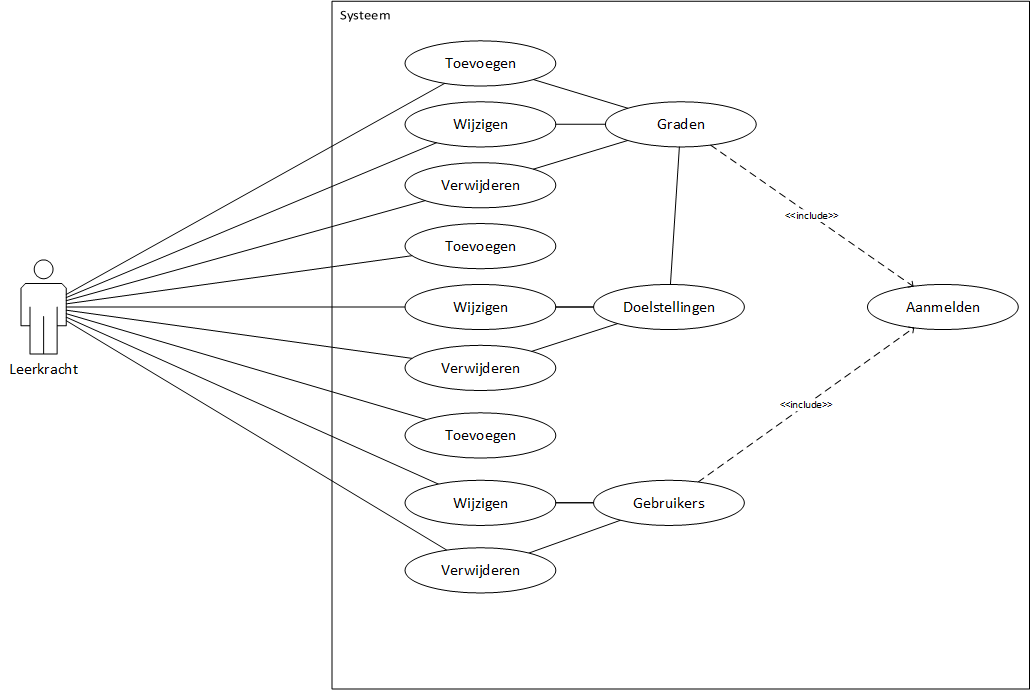
\includegraphics[width=\textwidth]{uc_beheerder}
  \caption{Usecase diagram voor de beheerder}
  \label{fig:usecase_beheerder}
\end{figure} 



%%%%%%%%%%%%%%%%%%%%%%%%%%%%%%%%%%%%%%%%%%%%%%%%%%%%%%%%%%%%%%%%%%%%%%%%%%%%%
%LEEKRACHT
%%%%%%%%%%%%%%%%%%%%%%%%%%%%%%%%%%%%%%%%%%%%%%%%%%%%%%%%%%%%%%%%%%%%%%%%%%%%%
\vspace{3em}
\subsection{Leerkracht}

% Werkgevers beheren
\begin{usecase}
    \addtitle{Use Case 4}{Werkgevers beheren} 
    \additemizedfield{Actoren}{
    	\item Leerkracht
    }
    \addscenario{Beschrijving}{
        \item[] \textbf{Hoofdscenario:} \\
        Leerkracht meldt zich aan via de webapplicatie. Leerkracht  kiest ``Werkgeversbeheer''. Lijst van werkgevers wordt getoond. De leerkracht kan werkgevers toevoegen, wijzigen en verwijderen. De informatie die ingevuld kan worden, kan terug gevonden worden in \ref{itm:werkgever_info}.
    }
\end{usecase}

% Werkgever koppelen
\begin{usecase}
    \addtitle{Use Case 5}{Werkgever koppelen} 
    \additemizedfield{Actoren}{
    	\item Leerkracht
    }
    \addscenario{Beschrijving}{
        \item[] \textbf{Hoofdscenario:} \\
          Leerkracht meldt zich aan via de webapplicatie. De Leerkracht gaat naar ``Werkgever toewijzen'' binnen het menu ``Werkgeversbeheer''. Men selecteert de gewenste leerling en de gewenste werkgever, en kiest ervoor deze te koppelen.\\
    }
\end{usecase}

% Contract genereren
\begin{usecase}
    \addtitle{Use Case 6}{Contract genereren} 
    \additemizedfield{Actoren}{
    	\item Leerkracht
    }
    \addscenario{Beschrijving}{
        \item[] \textbf{Hoofdscenario:} \\
          Leerkracht meldt zich aan via de webapplicatie. De Leerkracht gaat naar ``Contracten'' in het menu ``Werkgeversbeheer''. Het type contract wordt gekozen alsook de leerling waar een contract voor moet worden opgesteld. Info over de leerling en de werkgever worden automatisch ingevuld in het contract.\\
        \item[] \textbf{Alternatieve scenarios:} \\
        Er werd geen werkgever aan de leerling toegewezen (Use Case 5). De leerkracht krijgt hier een melding van, maar het contract wordt wel gegenereerd (zonder de informatie over de werkgever).\\
    }
\end{usecase}

\todo{VR: SSD + contracten}
% Puntenbeheer 
\begin{usecase}
    \addtitle{Use Case 7}{Puntenbeheer} 
    \additemizedfield{Primaire actor}{
    	\item Leerkracht
    } 
    \additemizedfield{Stakeholders en interests}{ 
        \item Leerkracht: Wilt een leerling op een gemakkelijke manier een score geven op een competentie/doelstelling.
    }
    \addfield{Preconditie}{
        De leerkracht moet aangemeld zijn. De opleidingen, klassen en leerlingen moeten bestaan.
    }
    \addfield{Postconditie}{
        De punten zijn opgeslagen. De aanpassing wordt weergegeven in de voortgang van de leerling. Doelstelling die drie keer is verworven, wordt in het grijs gezet wanneer er op een andere dag punten worden gegeven.}
    \addscenario{Hoofdscenario}{
        \item Leerkracht  kiest ``Puntenbeheer''.
        \item De leerkracht kiest in de eerste dropdown voor BGV.
        \item De leerkracht kiest in de tweede dropdown de opleiding.
        \item De leerkracht kiest in de derde dropdown de klas.
        \item De leerkracht kiest in de vierde dropdown de module/deelcertificaat.
        \item De leerkracht kiest op welke dag de competenties geëvalueerd werden.
        \item Het systeem toont een matrix met aan de linkerzijde de competenties die bij het gekozen deelcertificaat horen, en met bovenaan de leerlingen uit de gekozen klas. 
        \item De leerkracht selecteert de cel van de matrix die overeenkomt met de competentie en leerling waaraan hij een scoren wil geven.
        \item Onder de matrix toont het systeem een dropdown om de score (A, I, V) te geven en een veld om commentaar te schrijven (ter motivatie van de toegekende score).
        \item De leerkracht kiest in het dropdown A, I, V of leeg (als er geen score is gegeven).
        \item De leerkracht typt commentaar om de score te motiveren.
        \item De leerkracht klikt op ``Opslaan''.
        \item Het systeem behoudt de huidige pagina en de geselecteerde cel in het matrix wordt gedeselecteerd.
    }   
    \addscenario{Alternatieve scenarios}{
        \item[2.a] PAV: De leerkracht kiest voor PAV.
        \item[3.a] PAV: De leerkracht kiest voor de graad waarin hij een bepaalde klas wilt.
        \item[5.a] PAV: De leerkracht kiest voor het vakthema dat hij wilt beoordelen.
        \item[6.a] PAV: De leerkracht kiest op welke dag de doelstellingen geëvalueerd werden.
        \item[6.b] Score wijzigen: De leerkracht kiest de dag waarop hij de te wijzigen score gaf.
        \item[7.a] PAV: Het systeem geeft een matrix weer met aan de linkerzijde de doelstellingen die bij het gekozen vakthema horen, en met bovenaan de leerlingen uit de gekozen klas. 
        \item[7.b] Reeds beoordeelde doelstelling binnen een vakthema: De matrix wordt op bijna dezelfde manier weergegeven. Het enige verschil is dat de cel overeenkomstig met de reeds beoordeelde doelstelling is grijs gemaakt. Alleen op de dag waarop de score werd gegeven, is dit niet zo en kan de score dus worden gewijzigd.
        \item[7.c] Reeds behaalde doelstelling/competentie: De cel overeenkomstig met een doelstelling/competentie die de leerling reeds behaald (= drie keer verworven) heeft, is grijs. Enkel op de dagen dat ``V'' (verworven) als score werd toegekend, is dit niet het geval en kan de score dus gewijzigd worden.
        \item[8.a] Meerdere leerlingen en competenties/doelstellingen eenzelfde score en commentaar geven: De leerkracht selecteert alle gewenste cellen en vult onderaan de gemeenschappelijke score en commentaar in.
        \item[9.a] Verkeerde leerling punten gegeven: Selecteer de lege optie in de dropdown en deselecteer de cel in de matrix.
    }
    \addfield{Frequentie van voorkomen}{
        Bijna iedere dag dat er les wordt gegeven (2 keer per week)
    }
\end{usecase}

% !!!!!!!!!!! als je op een punt klikt krijg je een vakje met de commentaar te zien en voor pav het vakthema
% !!!!!!!!!!! toch nie mogelijk maken om in de voortgang punten aan te passen ? anders moet ge gaan kijken welke dag behaald en dan terug naar punten geven gaan wat veel stappen zijn
% Voortgang leerlingen (+rapporten)
\begin{usecase}
    \addtitle{Use Case 8}{Voortgang leerlingen} 
    \additemizedfield{Actoren}{
    	\item Leerkracht
    }
    \addscenario{Beschrijving}{
        \item[] \textbf{Hoofdscenario:} \\
        Leerkracht meldt zich aan via de webapplicatie. Leerkracht  kiest ``Voortgang leerlingen''. De leerkracht krijgt een lijst van leerlingen te zien waaraan hij/zij les geeft. De leerkracht kan per leerling de voortgang bekijken. De voortgang voor BGV en PAV staan in aparte tabs. De voortgang is een wekelijks overzicht van wanneer competenties(BGV)/doelstellingen(PAV) behaald zijn door deze leerling.\\
        \item[] \textbf{Alternatieve scenarios:} \\
        De leerkracht kan per leerling een rapport bekijken en dit afdrukken (in pdf formaat). Het rapport geeft een algemeen beeld van hoe de leerling het gedaan heeft a.d.v. staafdiagrammen (Per deelcertificaat/vakthema hoeveel competenties/doelstellingen ingeoefend en verworven zijn uit een totaal aantal te behalen competenties/doelstellingen).
    }
\end{usecase}

% Klasbeer
\begin{usecase}
    \addtitle{Use Case 9}{Klasbeheer} 
    \additemizedfield{Actoren}{
    	\item Leerkracht
    }
    \addscenario{Beschrijving}{
        \item[] \textbf{Hoofdscenario:} \\
        Leerkracht meldt zich aan via de webapplicatie. Leekracht kiest ``Mijn klassen''. De leerkracht krijgt een lijst van klassen te zien waaraan hij/zij les geeft. De leerkracht kan hier klassen toevoegen en verwijderen. De leerkracht kan een klas selecteren en dan leerlingen toevoegen of verwijderen in de tab ``Leerlingen''. De leerkracht kan een enkele leerling toevoegen maar ook meerdere via de knop ``Importeer leerlingen'' (De leerkracht kan zo bv. alle leerlingen van de 2de graad van een gekozen richting toevoegen aan zijn klas).
    }
\end{usecase}

%Klasbeheer -  Vakthema's
\begin{usecase}
    \addtitle{Use Case 10}{Klasbeheer -  Vakthema's} 
    \additemizedfield{Actoren}{
    	\item Leerkracht
    }
    \addscenario{Beschrijving}{
        \item[] \textbf{Hoofdscenario:} \\
        Leerkracht navigeert naar zijn klassen (Use case 9). De leerkracht selecteert een klas. De leerkracht selecteert de tab ``Vakthema's''. De leerkracht krijgt een lijst van vakthema's te zien. De leerkracht kan hier vakthema's toevoegen, verwijderen en aanpassen. Bij het invullen van de gegevens van een vakthema kan de leerkracht doelstellingen kiezen uit een lijst van alle doelstellingen. Naast iedere doelstelling staat een tellertje dat aangeeft hoe vaak deze doelstelling reeds aan een vakthema werd toegekend \footnotemark.\\
        \item[] \textbf{Alternatieve scenarios:} \\
        Leerkracht maakt een nieuw vakthema aan en vinkt aan dat het gaat om een remediëringstaak (deze telt niet bij tot het aantal keer een doelstelling voorkomt binnen de verschillende vakthema's). De leerkracht krijgt een lijst van leerlingen uit deze klas te zien. De leerkracht selecteert de leerlingen die in aanmerking komen voor deze remediëringstaak.
    }
\end{usecase}
\footnotetext{Iedere doelstelling 3 keer behaald moet worden, en dus 3 keer aan bod moet komen gedurende het schooljaar. Dankzij dit tellertje kan de leerkracht makkelijk bepalen welke doelstellingen nog in vakthema's aan bod moeten komen.}

\begin{figure}[H]
  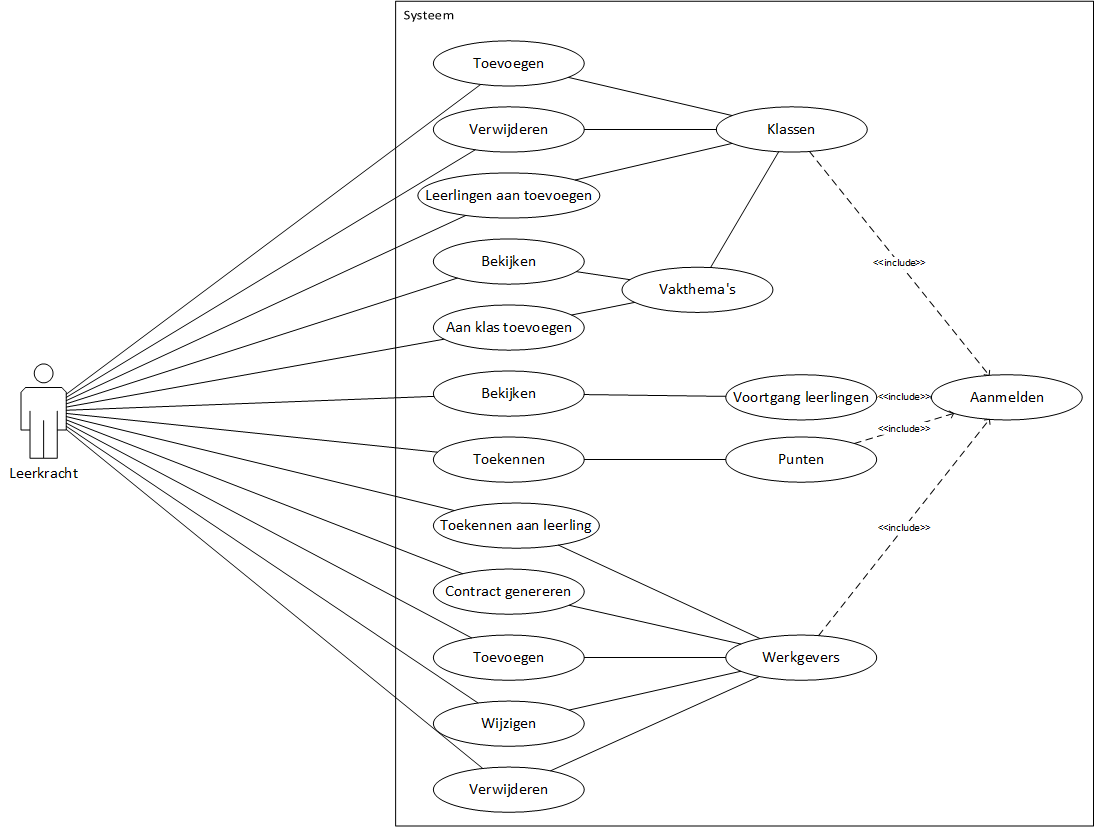
\includegraphics[width=\textwidth]{uc_leerkracht}
  \caption{Usecase diagram voor de leerkracht}
  \label{fig:usecase_leerkracht}
\end{figure}

%%%%%%%%%%%%%%%%%%%%%%%%%%%%%%%%%%%%%%%%%%%%%%%%%%%%%%%%%%%%%%%%%%%%%%%%%%%%%
%LEERLING
%%%%%%%%%%%%%%%%%%%%%%%%%%%%%%%%%%%%%%%%%%%%%%%%%%%%%%%%%%%%%%%%%%%%%%%%%%%%%

\newpage
\subsection{Leerling}
% Voortgang bekijken
% !!!!!!!!!!! als je op een punt klikt krijg je een vakje met de commentaar te zien en voor pav het vakthema
% !!!!!!!!!!! toch nie mogelijk maken om in de voortgang punten aan te passen ? anders moet ge gaan kijken welke dag behaald en dan terug naar punten geven gaan wat veel stappen zijn
\begin{usecase}
    \addtitle{Use Case 11}{Voortgang bekijken} 
    \additemizedfield{Actoren}{
    	\item Leerling
    }
    \addscenario{Beschrijving}{
        \item[] \textbf{Hoofdscenario:} \\
        Leerling meldt zich aan via de webapplicatie. Leerling kiest ``Voortgang''. De voortgang voor BGV en PAV staan in aparte tabs. Het systeem geeft een wekelijks overzicht van wanneer competenties(BGV)/doelstellingen(PAV) behaald werden door deze leerling.
    }
\end{usecase}

%Mobiele app - Tussentijd rapport
\begin{usecase}
    \addtitle{Use Case 12}{Mobiele app - Tussentijds rapport} 
    \additemizedfield{Actoren}{
    	\item Leerling
    }
    \addscenario{Beschrijving}{
        \item[] \textbf{Hoofdscenario:} \\
        Leerling meldt zich aan via de mobiele applicatie. Leerling kiest ``Tussentijds rapport''. Het tussentijds rapport is opgedeeld in drie tabs nl. ``Alle'', ``BGV'' en ``PAV'' voor meer overzichtelijkheid. Het tussentijds rapport geeft een algemeen beeld van hoe de leerling het gedaan heeft tot nu toe a.d.v. cirkeldiagrammen (Per deelcertificaat/vakthema hoeveel competenties/doelstellingen ingeoefend en verworven zijn uit een totaal aantal te behalen competenties/doelstellingen).
    }
\end{usecase}

\begin{figure}[H]
  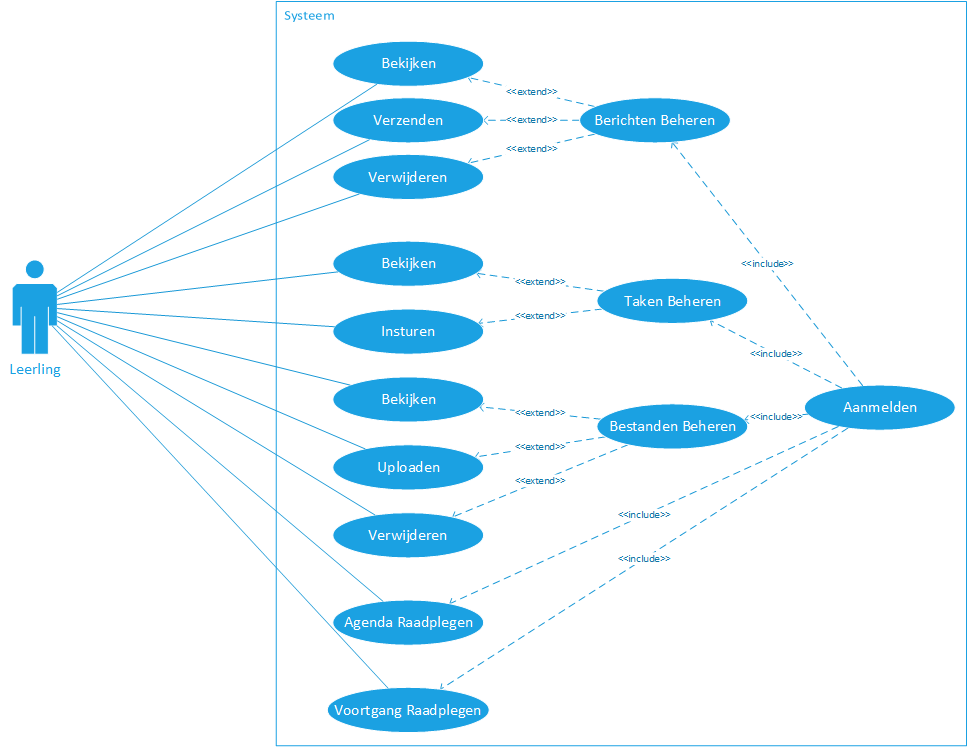
\includegraphics[width=\textwidth]{uc_leerling}
  \caption{Usecase diagram voor de leerling}
  \label{fig:usecase_leerling}
\end{figure}

%%%%%%%%%%%%%%%%%%%%%%%%%%%%%%%%%%%%%%%%%%%%%%%%%%%%%%%%%%%%%%%%%%%%%%%%%%%%%
%OUDER
%%%%%%%%%%%%%%%%%%%%%%%%%%%%%%%%%%%%%%%%%%%%%%%%%%%%%%%%%%%%%%%%%%%%%%%%%%%%%

\subsection{Ouder}
% Voortgang bekijken
\begin{usecase}
\addtitle{Use Case 13}{Voortgang bekijken} 
\additemizedfield{Actoren}{
	\item Ouder
}
\addscenario{Beschrijving}{
    \item[] \textbf{Hoofdscenario:} \\
    Ouder meldt zich aan via de webapplicatie. Ouder kiest kiest ``Voortgang''. De voortgang voor BGV en PAV staan in aparte tabs. Het systeem geeft een wekelijks overzicht van wanneer competenties(BGV)/doelstellingen(PAV) behaald zijn door het kind.\\
    \item[] \textbf{Alternatieve scenarios:} \\
    Indien de ouder meerdere kinderen heeft in de school, kan in een apart menu het gewenste kind geselecteerd worden.
}
\end{usecase}

%Mobiele app - Tussentijd rapport
\begin{usecase}
    \addtitle{Use Case 14}{Mobiele app - Tussentijds rapport} 
    \additemizedfield{Actoren}{
    	\item Ouder
    }
    \addscenario{Beschrijving}{
        \item[] \textbf{Hoofdscenario:} \\
        Ouder meldt zich aan via de mobiele applicatie. Ouder kiest ``Tussentijds rapport''. Het tussentijds rapport is opgedeeld in drie tabs nl. ``Alle'', ``BGV'' en ``PAV'' voor meer overzichtelijkheid. Het tussentijds rapport geeft een algemeen beeld van hoe dit kind het gedaan heeft tot nu toe a.d.v. cirkeldiagrammen (per deelcertificaat/vakthema hoeveel competenties/doelstellingen ingeoefend en verworven zijn uit een totaal aantal te behalen competenties/doelstellingen).\\
        \item[] \textbf{Alternatieve scenarios:} \\
        Indien de ouder meerdere kinderen heeft in de school, kan in een apart menu het gewenste kind geselecteerd worden.
    }
\end{usecase}

\begin{figure}[H]
  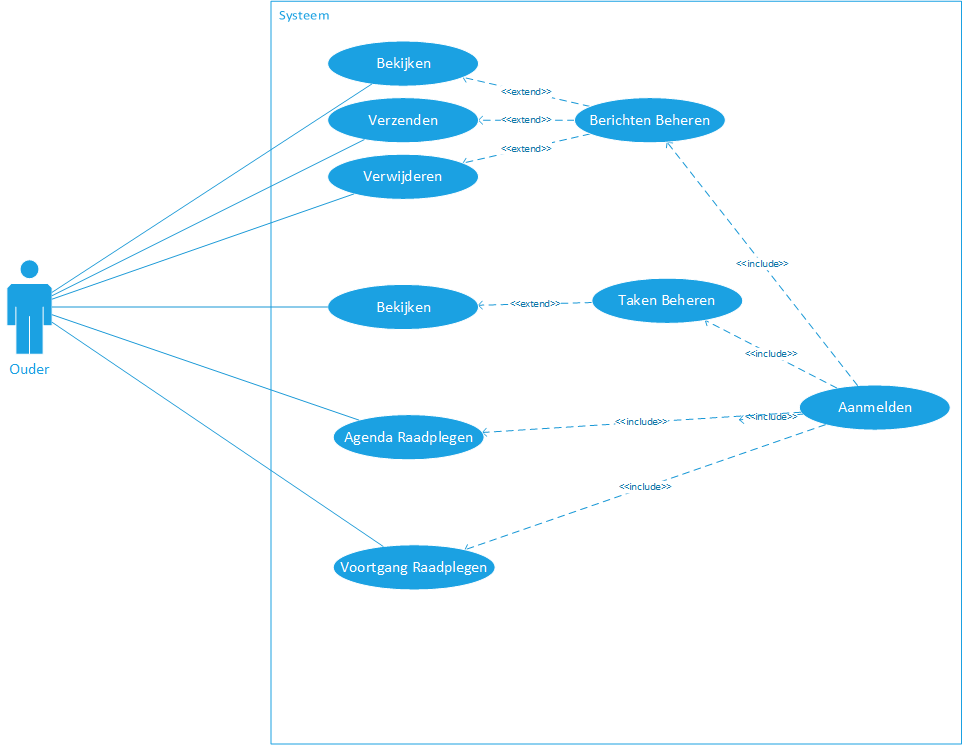
\includegraphics[width=\textwidth]{uc_ouder}
  \caption{Usecase diagram voor de ouder}
  \label{fig:usecase_ouder}
\end{figure}



\newpage
\section{Contracten}
\subsection{Gebruiker toevoegen}
\begin{tabularx}{\textwidth}{|l X|}
    \hline
    \textbf{Naam} & openUserManagement() \\
    \textbf{Verwijzingen} & \begin{itemize}[leftmargin=*]
        \item Use Case 1 - Gebruiker toevoegen
        \item Systeem Sequentie Diagram 1 - Gebruiker toevoegen
    \end{itemize}\\
    \textbf{Pre-condities} & De beheerder is aangemeld.\\
    \textbf{Post-condities} & \begin{itemize}[leftmargin=*]
        \item Voor iedere bestaande gebruiker in de database wordt een kopie van het User object aangemaakt (om aan de front-end terug te geven); creatie van instantie.
    \end{itemize}\\
    \hline
\end{tabularx}\\

\begin{tabularx}{\textwidth}{|l X|}
    \hline
    \textbf{Naam} & openCreateUser() \\
    \textbf{Verwijzingen} & \begin{itemize}[leftmargin=*]
        \item Use Case 1 - Gebruiker toevoegen
        \item Systeem Sequentie Diagram 1 - Gebruiker toevoegen
    \end{itemize}\\
    \textbf{Pre-condities} & De beheerder is aangemeld.\\
    \textbf{Post-condities} & \begin{itemize}[leftmargin=*]
        \item Er wordt een nieuwe instantie van User aangemaakt; creatie van instantie.
    \end{itemize}\\
    \hline
\end{tabularx}

\begin{tabularx}{\textwidth}{|l X|}
    \hline
    \textbf{Naam} & setUserType(leerlingType) \\
    \textbf{Verwijzingen} & \begin{itemize}[leftmargin=*]
        \item Use Case 1 - Gebruiker toevoegen
        \item Systeem Sequentie Diagram 1 - Gebruiker toevoegen
    \end{itemize}\\
    \textbf{Pre-condities} & \begin{itemize}[leftmargin=*]
        \item De beheerder is aangemeld.
        \item Er bestaat een instantie van User, user genaamd.
    \end{itemize}\\
    \textbf{Post-condities} & \begin{itemize}[leftmargin=*]
        \item user.type werd leerlingType; aanpassing attribuut.
    \end{itemize}\\
    \hline
\end{tabularx}\\

\begin{tabularx}{\textwidth}{|l X|}
    \hline
    \textbf{Naam} & setInfo(userinfo) \\
    \textbf{Verwijzingen} & \begin{itemize}[leftmargin=*]
        \item Use Case 1 - Gebruiker toevoegen
        \item Systeem Sequentie Diagram 1 - Gebruiker toevoegen
    \end{itemize}\\
    \textbf{Pre-condities} & \begin{itemize}[leftmargin=*]
        \item De beheerder is aangemeld.
        \item Er bestaat een instantie van User, user genaamd, waarvoor user.type gekend is.
    \end{itemize}\\
    \textbf{Post-condities} & \begin{itemize}[leftmargin=*]
        \item user.naam werd userinfo.naam; aanpassing attribuut.
        \item user.voornaam werd userinfo.voornaam; aanpassing attribuut.
        \item \dots  (alle attributen die persoonlijke informatie voorstellen, staan in \ref{itm:pers_info} opgesomd)
        \item user.username werd userinfo.username; aanpassing attribuut.
        \item user.password werd userinfo.password; aanpassing attribuut.
        \item user.email werd userinfo.email; aanpassing attribuut.
        \item user.pavklas werd userinfo.pavklas; aanpassing attribuut.
        \item user.bgvklas werd userinfo.bgvklas; aanpassing attribuut.
        \item user.inschrDatum werd userinfo.inschrDatum; aanpassing attribuut.
    \end{itemize}\\
    \hline
\end{tabularx}\\

\subsection{Puntenbeheer}
\begin{tabularx}{\textwidth}{|l X|}
    \hline
    \textbf{Naam} & openGrades() \\
    \textbf{Verwijzingen} & \begin{itemize}[leftmargin=*]
        \item Use Case 7 - Puntenbeheer
        \item Systeem Sequentie Diagram 2 - Puntenbeheer
    \end{itemize}\\
    \textbf{Pre-condities} & De leerkracht moet aangemeld zijn. De opleidingen, klassen en leerlingen moeten bestaan.\\
    \textbf{Post-condities} & \begin{itemize}[leftmargin=*]
        \item 
    \end{itemize}\\
    \hline
\end{tabularx}\\

\begin{tabularx}{\textwidth}{|l X|}
    \hline
    \textbf{Naam} & chooseSubject(BGV) \\
    \textbf{Verwijzingen} & \begin{itemize}[leftmargin=*]
        \item Use Case 7 - Puntenbeheer
        \item Systeem Sequentie Diagram 2 - Puntenbeheer
    \end{itemize}\\
    \textbf{Pre-condities} & De leerkracht moet aangemeld zijn. De opleidingen, klassen en leerlingen moeten bestaan.\\
    \textbf{Post-condities} & \begin{itemize}[leftmargin=*]
        \item 
    \end{itemize}\\
    \hline
\end{tabularx}\\

\begin{tabularx}{\textwidth}{|l X|}
    \hline
    \textbf{Naam} & chooseCourse(id) \\
    \textbf{Verwijzingen} & \begin{itemize}[leftmargin=*]
        \item Use Case 7 - Puntenbeheer
        \item Systeem Sequentie Diagram 2 - Puntenbeheer
    \end{itemize}\\
    \textbf{Pre-condities} & De leerkracht moet aangemeld zijn. De opleidingen, klassen en leerlingen moeten bestaan. Het vak moet reeds geselecteerd zijn.\\
    \textbf{Post-condities} & \begin{itemize}[leftmargin=*]
        \item 
    \end{itemize}\\
    \hline
\end{tabularx}\\

\newpage
\section{Scope}
\todo{NIEUW jens}
\subsection{Stap 1} % (MVP/minimal viable product) dit lijkt me misschien teveel maar je hebt al die dingen nodig voor puntenbeheerd fatsoenlijk werkt, ook best ieder deel opsplitsen ? zoals gebruikersbeheer opslplitsen in inschrijven , bewerken etc.
\begin{itemize} 
    \item Puntenbeheer
    \item Login Systeem
    \item Gebruikersbeheer
    \item Voortgang leerlingen Android-app
    \item Klasbeheer
\end{itemize}
\subsection{Stap 2}
\begin{itemize}
    \item Rapporten genereren
    \item Voortgang webapp 
\end{itemize}
\subsection{Stap 3}
\begin{itemize}
    \item wergeversbeheer
    \item bewerken graden en opleidingen
\end{itemize}


\section{Planning}
\begin{enumerate}
    \item \textbf{26/03} Analyse: bespreken van feedback van klant.
    \item \textbf{29/03} Analyse: feedback van klant verwerkt in verslag.
    \item \textbf{03/04} Analyse: feedback van onderwijsteam verwerkt in verslag.
    \item \textbf{04/04} Design: high-level UML, interactiediagrammen, .
    \item \textbf{25/04} Eerste iteratie: Puntenbeheer (met dummy data), loginsysteem, voortgang leerlingen in Android-app (met dummy data), gebruikersbeheer
    \item \textbf{25-29/04} Testing door gebruikers
    \item \textbf{23/05} Tweede iteratie: Voortgang leerlingen in webapp (en rapporten genereren), klassenbeheer, voortgang leerlingen in Android-app (met echte data), werkgeversbeheer (en contracten), bewerken van graden en opleidingen
\end{enumerate}


\section{Systeem evolutie}
Onderstaande modules zijn mogelijke uitbreidingen, geordend op prioriteit.
\begin{enumerate}
    \item Interne agenda waarin systeembeheerders lessen en algemene activiteiten kunnen inplannen. Extra functionaliteiten hierbinnen zijn de mogelijkheid om naar iCal te exporteren en meldingen te ontvangen in geval van last-minute wijzigingen.
    \item Een intern berichtensysteem waarmee gebruikers met elkaar kunnen communiceren. Hierin zouden de typische functionaliteiten zitten, zoals een bericht versturen, verwijderen, doorsturen, bijlages toevoegen.
    \item Een bestandsbeheersysteem waarin een gebruiker bestanden kan uploaden, en deze beheren (hernoemen, verwijderen, downloaden).
    \item Een takensysteem waarin leerkrachten een taak kunnen opleggen voor een bepaald vakthema. De leerlingen hebben de mogelijkheid om een bestand (= de taak) te uploaden.
\end{enumerate}


\section{Methodologie}
Er wordt per 2 aan eenzelfde module gewerkt, maar niet in de vorm van pair-programming, omdat dit praktisch moeilijk haalbaar is. Zo kunnen de teamleden elkaar snel verderhelpen in geval van moeilijkheden. Ook wisselen de teams regelmatig van module, zodat alle leden van het ontwikkelingsteam minstens een basiskennis hebben van alle code.


\newpage
\begin{appendices}
\section{Mockups webapplicatie}

\begin{figure}[H]
  \centerline{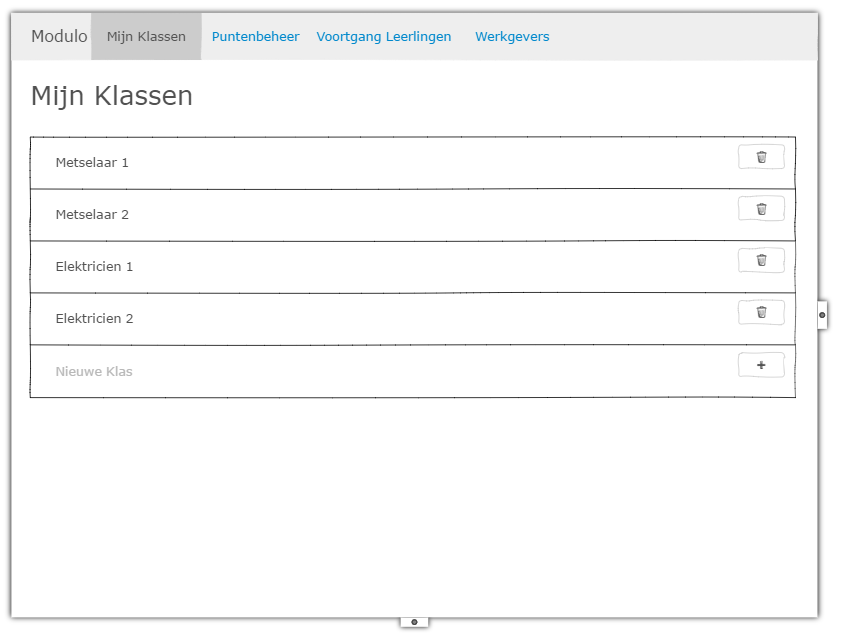
\includegraphics[width=\textwidth]{web_klassen}}
  \caption{Lijst van klassen van een leerkracht}
  \label{fig:web_klassen}
\end{figure}

\begin{figure}[H]
  \centerline{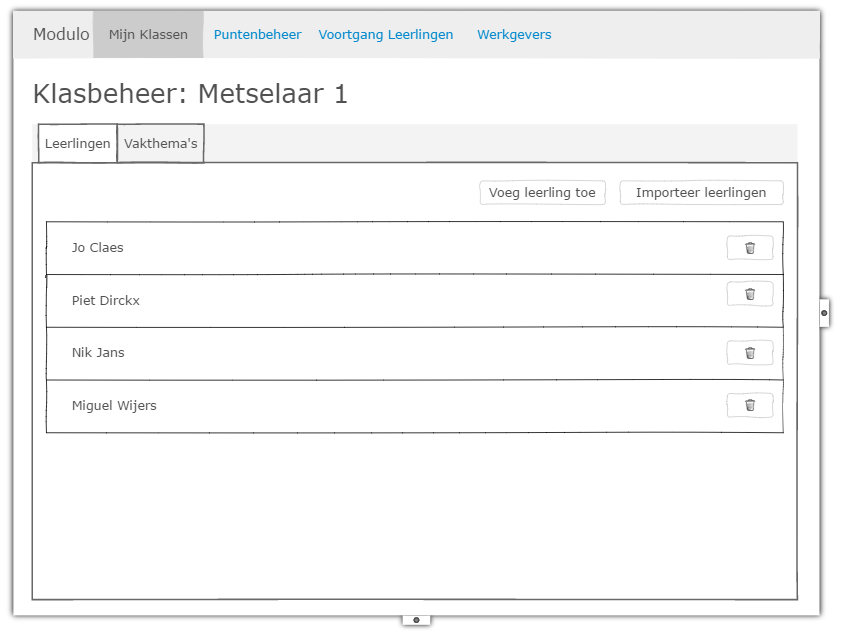
\includegraphics[width=\textwidth]{web_klasbeheer}}
  \caption{Beheer van een klas}
  \label{fig:web_klasbeheer}
\end{figure}

\todo{toevoegen datum selectie}
\begin{figure}[H]
  \centerline{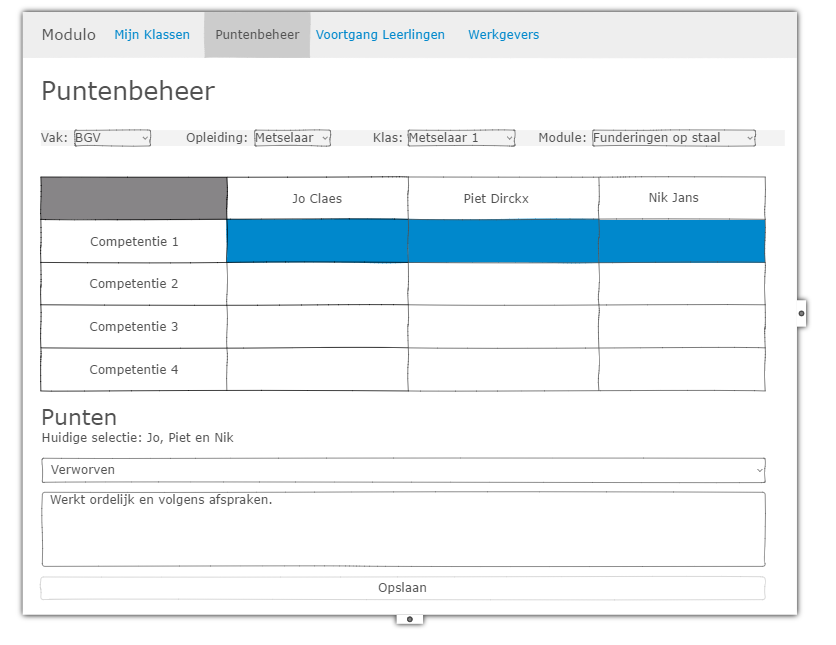
\includegraphics[width=\textwidth]{web_punten}}
  \caption{Opzoeken en toekennen van punten}
  \label{fig:web_punten}
\end{figure}

\begin{figure}[H]
  \centerline{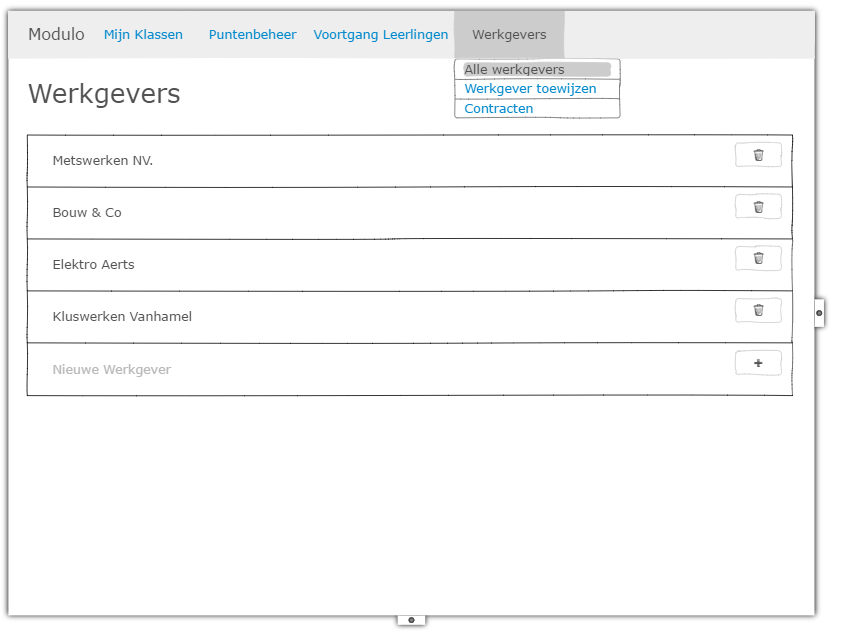
\includegraphics[width=\textwidth]{web_werkgevers_dropdown}}
  \caption{Dropdown werkgevers}
  \label{fig:web_werkgevers_dropdown}
\end{figure}

\newpage
\section{Mockups mobiele applicatie}

\begin{figure}[H]
  \centerline{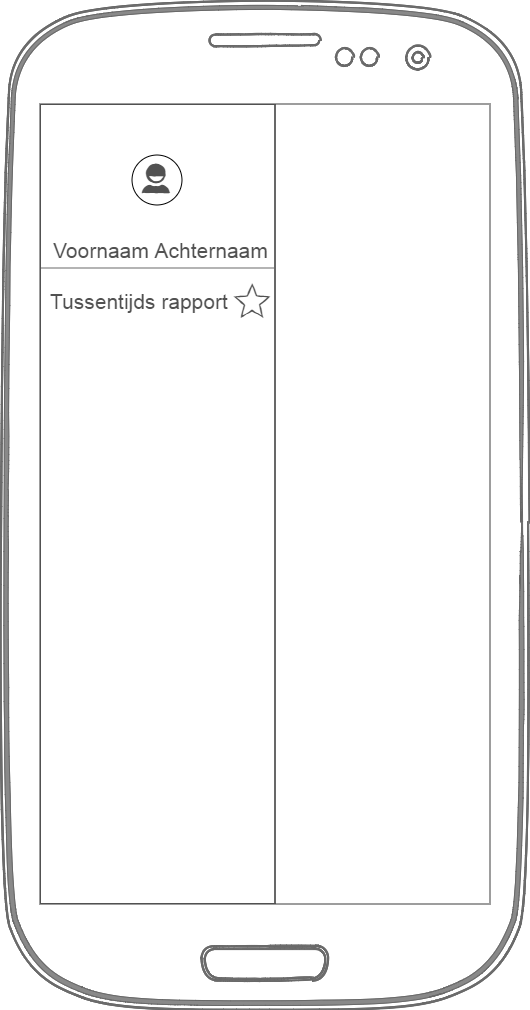
\includegraphics[width=\textwidth*4/5]{MobieleApp/leerling_view}}
  \caption{Menu voor leerlingen}
  \label{fig:mobiel_leerling}
\end{figure}

\newpage
\begin{figure}[H]
  \centerline{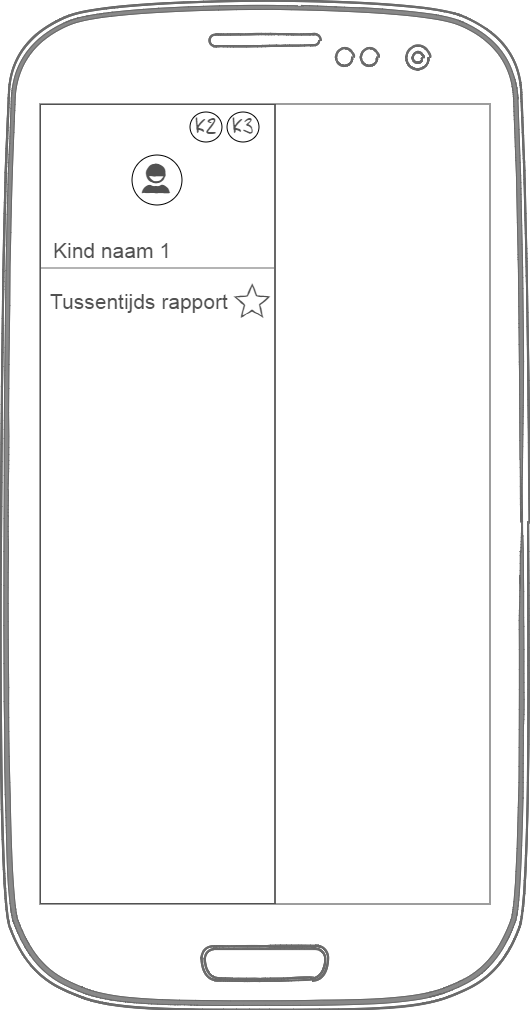
\includegraphics[width=\textwidth*4/5]{MobieleApp/ouders_view}}
  \caption{Menu voor ouders}
  \label{fig:mobiel_ouder}
\end{figure}

\newpage
\begin{figure}[H]
  \centerline{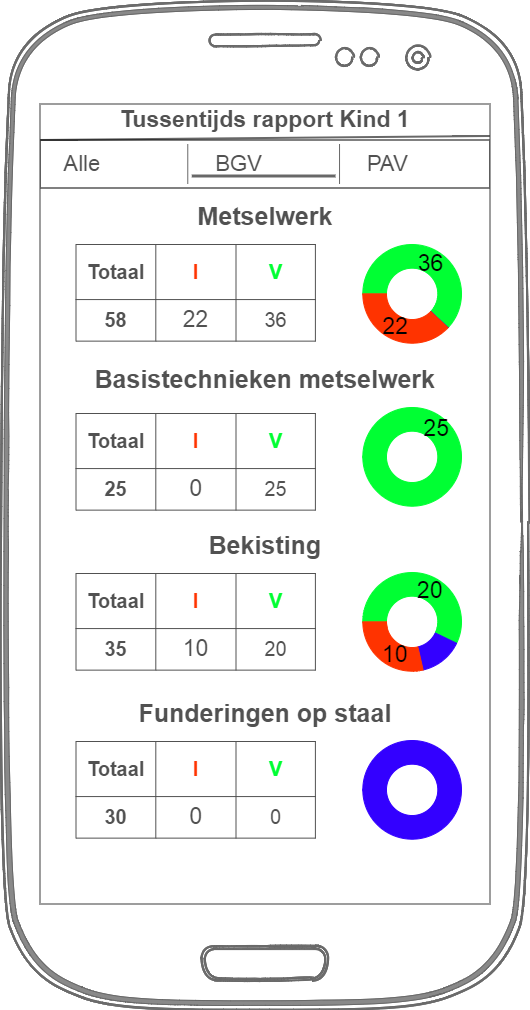
\includegraphics[width=\textwidth*4/5]{MobieleApp/tussentijds_rapport}}
  \caption{Tussentijds rapport}
  \label{fig:mobiel_tussentijds_rapport}
\end{figure}


\end{appendices}

\newpage
\bibliography{Referenties}
\bibliographystyle{unsrt}

\end{document}

%  Gebruikersbeheer
%  Mijn klassen
%       Lijst van klassen (en toevoegen, verwijderen klassen))
%           klasbeheermenu (leerlingen toevoegen/verwijderen, vakthema's toevoegen (met tellertjes per doelstelling die aangeven hoeveel keer een doelstelling reeds in de vakthema's zit), optie bij vakthema toevoegen om er een remediëringstaak van te maken en geeft lijst van leerlingen, vakthema's verwijderen)
%
%  Puntenbeheer
%       bgv / pav
%           opleiding / graad
%               klas / klas
%                   bgv -> deelcertificaat / pav -> vakthema
%
%  Voortgang leerlingen
%       voortgang per leerling
%       rapporten afdrukken
%
%  Werkgeversbeheer
%       contracten
%       werkgevers
%       werkgever toewijzen
%
%  graden/opleidingen (competenties/doelstellingen)
%       om te bewerken kiezen welk vak, dan graad/opleding, deelcertificaat en dan wijzigen 

% indien we een doelstelling of competentie 3keer verworven hebben dan gaan we alle dagen uitgrijzen behalve de dage waarop de doelstelling verworven is zodat we deze nog kunnen aanpassen

F